\subsubsection{Quinto periodo (2024/01/16 - 2024/02/12)}
\subsubsubsection{Planning}
\subsubsubsubsection*{Attività pianificate}
Nel corso dello $\textit{sprint}_G$, il team \emph{RAMtastic6} ha previsto un periodo di sospensione parziale delle attività di circa due settimane, dal 22/1/2024 fino al 5/2/2024.
Gli obiettivi posti per lo $\textit{sprint}_G$ sono stati i seguenti:
\begin{itemize}
    \item Implementare una prima versione di ricerca e $\textit{prenotazione}_G$ del ristorante all'interno del Poc;
    \item Completare il documento \emph{Analisi dei Requisiti} aggiungendo i requisiti funzionali.
\end{itemize}

\subsubsubsubsection*{Preventivo}
\begin{table}[H]
    \centering
\begin{spreadtab}{{tabular}{|c|c|c|c|c|c|c|c|}}
    \hline
    @\textbf{Membro} & @\textbf{Re} & @\textbf{Amm} & @\textbf{An} & @\textbf{Progr} & @\textbf{Proge} & @\textbf{Ve} & @\textbf{Totale} \\
    \hline
    @ Samuele V.   & 0          & 0          & 3         & 0          & 0     & 0     & sum(b2:g2) \\
    @ Leonardo B.  & 4         & 0          & 0        & 0        & 0     & 0.5   & sum(b3:g3) \\
    @ Riccardo Z.  & 0          & 0          & 0          & 5.5          & 0     & 0   & sum(b4:g4) \\
    @ Davide B.    & 0          & 0          & 4       & 0       & 0     & 0     & sum(b5:g5) \\
    @ Michele Z.   & 0          & 2          & 0         & 0          & 0     & 0     & sum(b6:g6) \\
    @ Filippo T.   & 0          & 0          & 0         & 0          & 0     & 4     & sum(b7:g7) \\
    \hline
    @\textbf{Ore totali} & sum(b2:b7) & sum(c2:c7) & sum(d2:d7) & sum(e2:e7) & sum(f2:f7) & sum(g2:g7) &  sum(b8:g8)\\
    \hline
    @\textbf{Costo totale} & 30*b8 & 20*c8 & 25*d8 & 15*e8 & 25*f8 & 15*g8 & sum(b9:g9)\\
    \hline
\end{spreadtab}
    \caption{Preventivo orario ed economico parziale per il quinto periodo, in base al ruolo}
    \label{tab:prev_rtb}
    \vspace{5mm}
    \textbf{Legenda:} \textit{Re} = Responsabile, \textit{Amm} = Amministratore, \textit{An} = Analista, \textit{Progr} = Programmatore, \textit{Proge} = Progettista, \textit{Ve} = Verificatore
\end{table}
\begin{figure}[H]
  \centering
  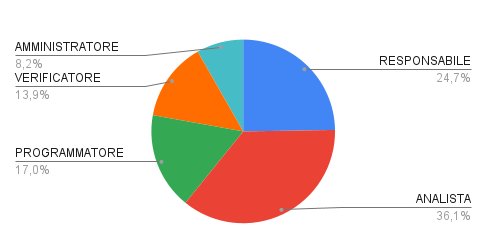
\includegraphics[width=0.6\linewidth]{grafici/5_periodo_torta.png}
  \caption{Ripartizione dei costi per ruolo nel $5^\circ$ periodo}
        \vspace{10mm}
  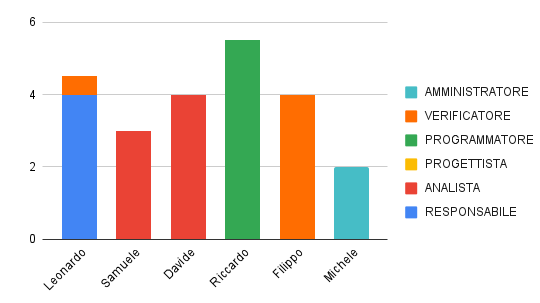
\includegraphics[width=0.7\linewidth]{grafici/5_periodo_istogramma.png}
  \caption{Ore preventivate per ciascuna persona nel $5^\circ$ periodo}
\end{figure}
\subsubsubsection{Review}
\subsubsubsubsection*{Attività svolte}
Per quanto riguarda l'Analisi dei Requisiti:
\begin{itemize}
    \item Sono state apportate correzioni a degli UC esistenti;
    \item Si è creata la sezione requisiti funzionali nel documento \emph{Analisi dei Requisiti}.
\end{itemize} 
\subsubsubsubsection*{Consuntivo}
\begin{table}[H]
    \centering
\begin{spreadtab}{{tabular}{|c|c|c|c|c|c|c|c|}}
    \hline
    @\textbf{Membro} & @\textbf{Re} & @\textbf{Amm} & @\textbf{An} & @\textbf{Progr} & @\textbf{Proge} & @\textbf{Ve} & @\textbf{Totale} \\
    \hline
    @ Samuele V.   & 0          & 0          & 3.75         & 0          & 0     & 0     & sum(b2:g2) \\
    @ Leonardo B.  & 3.25         & 0          & 0        & 0        & 0     & 0.75    & sum(b3:g3) \\
    @ Riccardo Z.  & 0          & 0          & 0          & 5.75          & 0     & 0   & sum(b4:g4) \\
    @ Davide B.    & 0          & 0          & 4.5       & 0       & 0     & 0     & sum(b5:g5) \\
    @ Michele Z.   & 0          & 1.17          & 0         & 0          & 0     & 0     & sum(b6:g6) \\
    @ Filippo T.   & 0          & 0          & 0         & 0          & 0     & 2.42     & sum(b7:g7) \\
    \hline
    @\textbf{Ore totali} & sum(b2:b7) & sum(c2:c7) & sum(d2:d7) & sum(e2:e7) & sum(f2:f7) & sum(g2:g7) &  sum(b8:g8)\\
    \hline
    @\textbf{Costo totale} & 30*b8 & 20*c8 & 25*d8 & 15*e8 & 25*f8 & 15*g8 & sum(b9:g9)\\
    \hline
    %@\textbf{Diff. preventivo} & 0 & 0 & 0 & 1 & 0 & 0 & sum(b10:g10)\\
    %\hline
\end{spreadtab}
    \caption{Consuntivo orario ed economico parziale per il quinto periodo, in base al ruolo}
    \label{tab:prev_rtb}
    \vspace{5mm}
    \textbf{Legenda:} \textit{Re} = Responsabile, \textit{Amm} = Amministratore, \textit{An} = Analista, \textit{Progr} = Programmatore, \textit{Proge} = Progettista, \textit{Ve} = Verificatore
\end{table}
\subsubsubsection{Retrospective}
In questo periodo sono state riscontrate delle problematiche nello sviluppo dei casi d'uso; in particolare è stata rivista la gerarchia degli attori e si è cercato di dare un senso atomico al loro nome. Inoltre, si è riscontrato il rischio \nameref{ro:3} in quanto diversi membri del gruppo erano impegnati con la sessione d'esame. 